% Datei: redakteurin.tex
% Kodierung: UTF-8


% Aufbauend auf der bisherigen Dokumentation von Heiko wird dargestellt,
% wie der Gemeindezeitungsgenerator benutzt werden kann. Mir (cl) ist
% es dabei wichtig, daß ich im Detail nachvollziehen kann, was bei 
% welchem Befehl passieren soll und das auch dokumentiere.
% 
% Mir schwebt vor, dass unterschiedliche Rollen unterschiedliche Details
% interessieren, z.B. beim Einstellen, bei der Korrektur oder aber beim
% abschließenden Formatieren. 
% 

\documentclass[12pt,a4paper,twoside]{article}% Standard für endgültige Gemeindeinformation
%\documentclass[12pt,a4paper,draft,twoside]{article}% mit Kennzeichnung von overfull hbox
%\usepackage{pxfonts} %Adobe Palatino - TypeI-Zeichensatz
\usepackage[ngerman]{babel}%u.a. korr. Trennung ab 2010
\usepackage{graphicx}
\usepackage{layout}%ermöglicht die Anzeige des SeitenLayouts via \layout*
\usepackage{ucs}%utf8-zusatz
\usepackage[utf8x]{inputenc}%utf8 - Zeichensatz.
\usepackage{textcomp}
\usepackage{amsmath}%Mathematik
\usepackage{amssymb}%Mathematik
\usepackage{multicol}%Mehrspaltensatz
%\usepackage{fancyhdr}%Kopf/Fusszeilen-Layout
\usepackage{array}%Erweiterung Tabellenumgebung
\usepackage{pifont}%Symbolfont : \ding{0..255} bzw. \begin dinglist{0..255}Erweiterung Tabellenumgebung
%\usepackage{wrapfig}%Textboxen etc.
\usepackage[right]{eurosym} %Eurosymbol \EUR{50,-} bzw \euro{}
%
\usepackage{tabularx}% ermöglicht mehr Anpassungen bei Tabellen, z.B. die folgende
\newcolumntype{L}[1]{>{\raggedright\arraybackslash}p{#1}}% linksbündige Spalten mit Breitenangabe 
% Navigation innerhalb des PDF (muss das letzte Paket sein): 
%.aux darf nicht gelöscht werden, um das Paket nutzen zu können
\usepackage{hyperref}
\urlstyle{same}% use the same style for URLs, too (not with a mono-spaced font)
\hypersetup{
    %bookmarks=true,          % show bookmarks bar? - Warning: `bookmarks' has already been used,
    unicode=false,            % non-Latin characters in Acrobat’s bookmarks
    pdftoolbar=true,          % show Acrobat’s toolbar?
    pdfmenubar=true,          % show Acrobat’s menu?
    pdffitwindow=false,       % window fit to page when opened
    pdfstartview={FitH},      % fits the width of the page to the window
    pdftitle={Benutzerdokumentation zum Berg CMS}, % title
    pdfauthor={Christian Leutloff},   % author
    pdfsubject={Dokumentation - Redakteur/-in},   % subject of the document
    %pdfcreator={Creator},    % creator of the document
    pdfproducer={Christian Leutloff}, % producer of the document
    %pdfkeywords={keyword1} {key2} {key3}, % list of keywords
    pdfnewwindow=true,        % links in new window
    colorlinks=true,          % false: boxed links; true: colored links
    linkcolor=black,          % color of internal links
    citecolor=black,          % color of links to bibliography
    filecolor=black,          % color of file links
    urlcolor=black            % color of external links
}


%*********************
%...Seitengestaltung 
%*********************
\setlength{\hoffset}{-15mm}%..........................Korrektur des Druckbereichs horizontal
\setlength{\voffset}{-30mm}% .........................Korrektur des Druckbereichs vertikal
\setlength{\emergencystretch}{4em}%...................Randausgleich Blocksatz
\setlength{\textwidth}{190mm}%........................TextboxBreite(A4=210)
\setlength{\textheight}{265mm}%.......................TextboxHöhe(A4=297)
\setlength{\parindent}{0mm}%..........................Absatz-Einrückung 1.Zeile
%\setlength{\parskip}{1.0ex plus 0.5ex minus 0.5ex}%...VarioAbsatzAbstände
\setlength{\parskip}{1.0ex plus 0.8ex minus 0.5ex}%...VarioAbsatzAbstände
\setlength{\columnsep}{7mm}%..........................SpaltenZwischenraum
\setlength{\columnseprule}{0.2pt}%....................Spaltentrennlinie
\setlength{\oddsidemargin}{0mm}%......................linker Rand ungerade(rechte) Seiten
\setlength{\evensidemargin}{0mm}%.....................linker Rand gerade(linke) Seiten
\setlength{\footskip}{8mm}%...........................Abstand: unterer Textbox - Seitenrand
\setcounter{secnumdepth}{-2}%.........................AschnittsNummerierungstiefe - Abschalten
\setcounter{tocdepth}{2}%.............................Inhaltsverzeichnistiefe festlegen
\pagestyle{plain}%....................................Seitenstil: Seitennummerierung zentral/unten


%%%%%%%%%%%%%%%%%%%%%%%%%%%%%%%%   Fusstext   %%%%%%%%%%%%%%%%%%%%%%%%%%%%%%%%

%------------------------------------
\begin{document}
%------------------------------------
%\layout*%..........................................Seitenspiegel zu Testzwecken einblenden

Stand: 19. Mai 2016 (erzeugt \today) 


In diesem Dokument wird der Einsatz des Berg CMS zur Erstellung der 
Gemeindeinformation/Pfarrbrief o.ä. aus Sicht einer Redakteurin oder Redakteurs sowie bei der 
Korrektur dargestellt. Zur Erstellung der Gemeindeinformation werden die Artikel 
in einer Datenbank eingegeben. Dann werden die Artikel automatisch zusammengestellt und gesetzt.
Das Ergebnis ist eine PDF-Datei, die dann von der Druckerei vervielfältigt wird.
Das gesamte Redaktionssystem wird nur mit einem Web-Browser, wie dem 
Mozilla Firefox, bedient.

Nach der Eingabe der Start-URL, \url{http://bergcms.local/cgi-bin/brg/berg.pl}, erscheint die folgende
Seite. Der Hostname "`bergcms.local"' muss durch den Servernamen ersetzt werden, auf dem das Berg CMS installiert wurde.


\begin{figure}[h]
\begin{center}
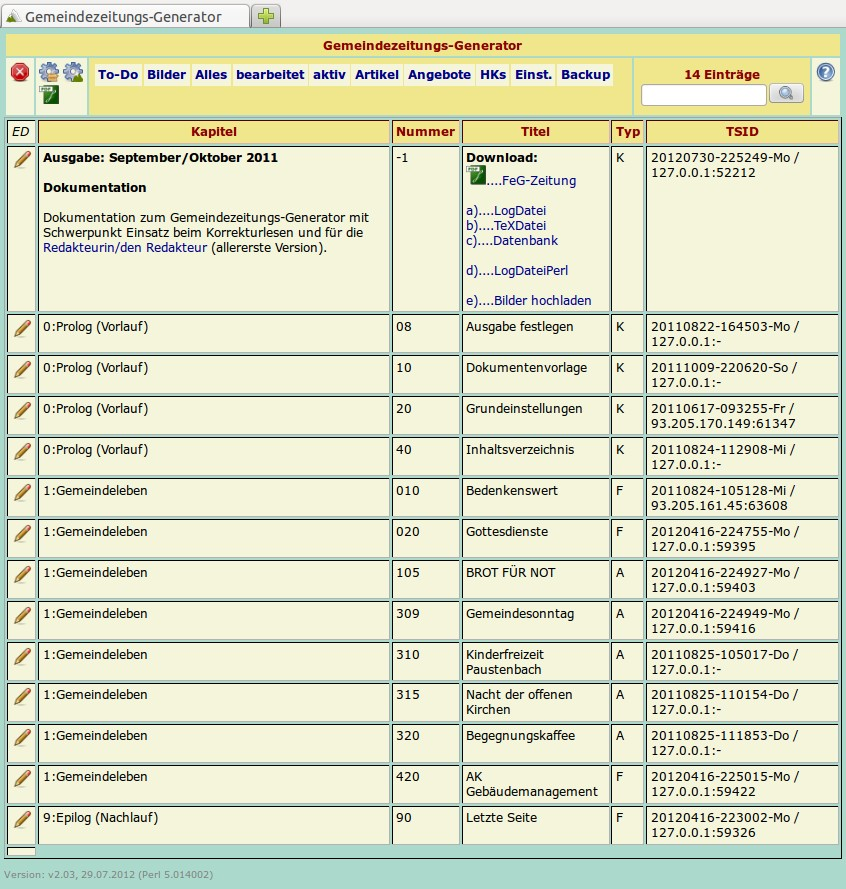
\includegraphics[width=0.65\linewidth]{webgui_startseite.jpeg}
\end{center}
\caption{Startseite}
\end{figure} 

Die Startseite ist unterteilt in einen Kopfbereich und eine große Tabelle.
In der Tabelle sind alle Artikel aus der zugrundeliegenden Datenbank aufgelistet.
Der Kopfbereich stellt verschiedene Teilfunktionen des Gemeindezeitungsgenerators bereit. 
Zum einen ermöglicht er die Zusammenstellung der Gemeindeinformation zu starten und das Ergebnis
herunterzuladen. Zum anderen
 ermöglicht die Navigation zu verschiedenen Teilansichten, die 
nur noch bestimmte Artikel auflisten, oder zur Suche und zu den Hilfetexten. 

\begin{figure}[h]
\begin{center}
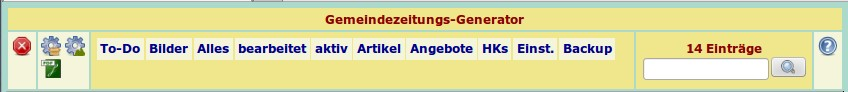
\includegraphics[width=0.9\linewidth]{webgui_kopfbereich.jpeg}
\end{center}
\caption{Navigation}
\end{figure} 

Die folgende Tabelle 
listet die verschiedenen Funktionen auf.
%  stop.jpeg
% 
\includegraphics[height=2ex]{icons/berg.jpeg}
\begin{center}                 
\begin{tabular}{|l|p{13cm}|}
\hline

\includegraphics[height=4ex]{icons/abort.jpeg} & Rückkehr zur Startseite. \\ \hline\hline


\includegraphics[height=4ex]{icons/ark.jpeg} &  Zusammenstellung der Gemeindeinformation starten.  \\ \hline

\includegraphics[height=4ex]{icons/maker.jpeg} & Zusammenstellung der Gemeindeinformation starten und direkt die Protokolldateien anzeigen. \\ \hline

\includegraphics[height=4ex]{icons/pdfreaders.jpeg} & Zusammengestellte Gemeindeinformation als PDF herunterladen. \\ \hline\hline

 
To-Do & Die Aufgabenliste des Redaktionsteams. \\ \hline


Bilder & Bilder in das Redaktionssystem hochladen. \\ \hline
 
Alles & Alle Artikel der Datenbank. Dies ist auch die Startseite. \\ \hline

bearbeitet & Die zuletzt bearbeiteten Artikel. Diese Information kann genutzt werden, um zu sehen woran zuletzt gearbeitet wurde. \\ \hline

aktiv & Alle Teildokumente, die in dieser Ausgabe der Gemeindeinformation erscheinen sollen.   \\ \hline

Artikel & Alle Artikel der Gemeindeinformation, ohne die kontinuierlichen Rubriken. Diese Ansicht ist empfehlenswert zum Korrekturlesen.\\ \hline

%Angebote& Alle Artikel mit Angeboten \\ \hline
%HKs &  Artikel zu den Hauskreisen \\ \hline
Einst. & Artikel mit Einstellungen  \\ \hline
Backup& Zum Backup, in dem die zuletzt veränderten Artikel hinterlegt sind und von dort wiederhergestellt werden können. \\ \hline


\includegraphics[height=4ex]{icons/search.jpeg} & Suche in allen Artikel der Datenbank. \\ \hline\hline


\includegraphics[height=4ex]{icons/help.jpeg} & Seite mit Verweisen auf die verschiedenen Protokolldateien,
 die beim Zusammenstellen der Gemeindeinformation erzeugt werden, und den Hilfedokumenten. \\ \hline

\end{tabular} 
\end{center}


\begin{figure}[h]
\begin{center}                 
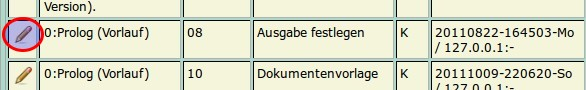
\includegraphics[width=0.6\linewidth]{webgui_artikelauswahl.jpeg}
\end{center}                 
\caption{Artikel in einer der Tabellenansichten zur Bearbeitung auswählen}
\end{figure} 


Zum Bearbeiten eines Artikels dient das "`Edit"'-Symbol 
\includegraphics[height=2ex]{icons/pencil.jpeg}.
Nach dem Anklicken erscheint der Artikel mit Überschrift und dem eigentlichen Text.


\begin{figure}[h]
\begin{center}                 
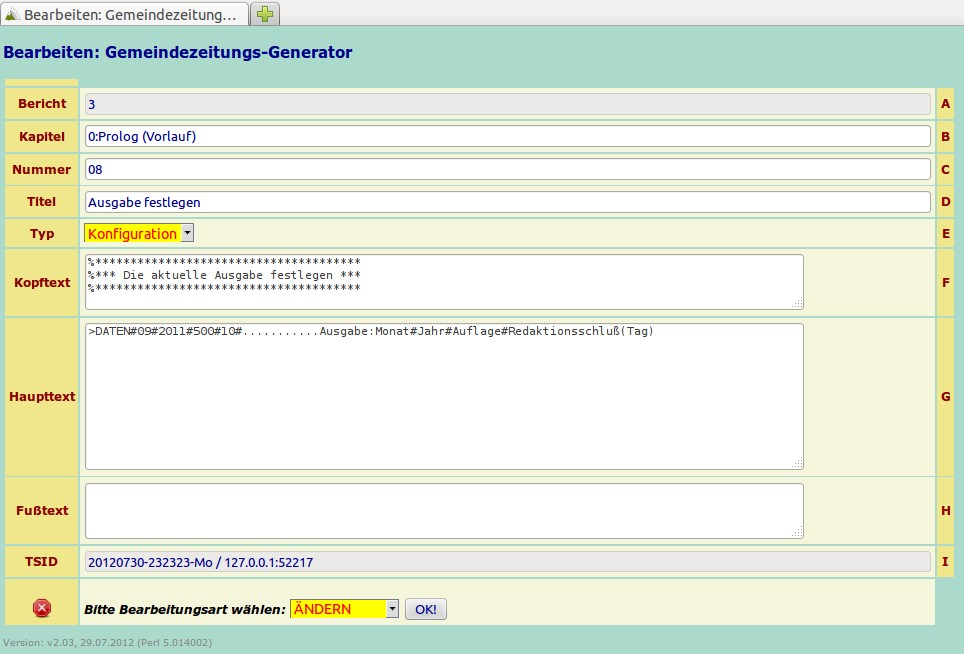
\includegraphics[width=0.9\linewidth]{webgui_bearbeiten.jpeg}
\end{center}                 
\caption{Artikel bearbeiten}
\end{figure} 

Um die Änderungen zu speichern, reicht es aus den "`OK"'-Button 

\includegraphics[height=2ex]{icons/aendern.jpeg} zu klicken. 

Sollen die bisherigen Änderungen verworfen werden oder wurden keine Änderungen 
vorgenommen, so wird der Vorgang mit dem Abbrechen-Symbol

\includegraphics[height=2ex]{icons/abort.jpeg}
beendet.


\end{document}


% weiteres:

Fehlende Bilder werden durch einen entsprechenden Hinweis im Text gekennzeichnet.

Die Backup-Datenbank wird neu angelegt, wenn sie nicht existiert.

Eine Tabelle ohne Rahmen bekommst du, in dem du | weglässt. Die erste Zeile einer Tabelle ist fest als Überschrift definiert. 

